\documentclass{book}
%\usepackage{epsf}
\usepackage{graphicx}
%\usepackage[dvipdfmx]{graphicx}
\usepackage{caption}
\usepackage{subcaption}
\usepackage{hyperref}
%\documentstyle[epsf]{jbook}
%\documentstyle[12pt,epsf]{jbook}

\title{RIKEN AICS\\
       Annual Report FY2016\\
      AICS Research Activities}
\author{}

%\setlength{\unitlength}{1cm}
%\setlength{\textwidth}{17cm}
%\setlength{\textheight}{24cm}
%\setlength{\oddsidemargin}{-1cm}
%\setlength{\evensidemargin}{-1cm}
%\setlength{\topmargin}{-0.5cm}

\begin{document}

\maketitle

\section*{Preface}

\newpage

\section*{Organization}


\tableofcontents

\part{Research Division}

\chapter{HPC Programming Framework Research Team}

\section{Members}

\begin{itemize}
  \item[] Naoya Maruyama (Team Leader)
  \item[] Motohiko Matsuda (Research Scientist)
  \item[] Shinichiro Takizawa (Research Scientist)
  \item[] Mohamed Wahib (Postdoctoral Researcher)
  \item[] Keisuke Fukuda (Research Associate)
  \item[] An Huynh (Student Trainee)
  \item[] Satoshi Matsuoka (Senior Visiting Scientist)
  \item[] Tomoko Nakashima (Assistant)
  \item[] Aya Motohashi (Assistant)
\end{itemize}


\section{Research Activities}

We develop high performance, highly productive software stacks that aim to simplify development of highly optimized, fault-tolerant computational science applications on current and future supercomputers, notably the K computer. Our current focus of work includes large-scale data processing, heterogeneous computing, and fault tolerance. A major ongoing project in our group will deliver a MapReduce runtime that is highly optimized for the intra- and inter-node architectures of the K computer as well as its peta-scale hierarchical storage systems. Another major project focuses on performance and productivity in large-scale heterogeneous systems. Below is a brief summary of each project.


\section{Research Results and Achievements}

\subsection{KMR}

\subsubsection{A Scalable Multi-Granular Data Model for Data Parallel Workflows}

A wide range of scientific applications, including weather modeling, molecular dynamics and astrophysics, are run on large scale parallel computing systems.
Obtaining scientific insights, however, requires executing those applications multiple times typically with different parameter configurations with different applications running concurrently, composing parallel workflows.
Tasks in such a workflow typically run with multiple processes but the degree of parallelism often varies, resulting in the different numbers of tasks with the different numbers of processes.
For example, a climate simulation with data assimilation can be realized by an ensemble execution of a climate model with different input values, followed by statistical adjustment of physical properties using real observation data.
In the former phase, each task of the climate model is a parallel application with the whole simulation region split among parallel processes.
In the latter phase, a statistical analysis on each grid point in the simulation region is run using all ensemble output and observation data of the point.
Though a task in the former phase requires multiple processes, a task in the latter phase only requires a single process but the number of tasks is much larger.
Moreover, processes in each phase have completely different data access patterns.
Appropriate data decomposition and arrangement to processes are required between these two phases.
Otherwise, performance degradation occurs due to unnecessary remote access.

To efficiently execute these applications, it is necessary to satisfy requirements for degree of parallelism, number of ensembles and data access pattern of all tasks that compose the applications.
Application developers have to take the following three steps to write code that satisfies the above requirements for each task: (1) allocate enough number of processes to each ensemble, (2) decompose input data and arrange them to processes and (3) execute the task.
Coding of these steps is highly troublesome and error-prone because data arrangement in (2) requires correct decomposition and transfer of the input by considering data access pattern.
Moreover, as the implementation effort is in proportion to the number of tasks in a workflow, it becomes even worse for larger applications.
Though the above problem is a common issue for applications irrespective of science fields, there are no common effective solutions and the reality is that developers have to hand-write the troublesome codes.

To solve the problem, we propose a multi-view data model that allows the user to create multi-dimensional arrays with adaptive granularities of decomposition to achieve efficient execution of data parallel workflows.
Our framework conducts data arrangement and affinity-aware task scheduling as specified by the user with straightforward programming constructs (Fig.~\ref{takizawa_sample}).
We present a prototype implementation for distributed-memory parallel systems using MPI with APIs for C, C++, and Fortran.
A case study using a lattice QCD code called BQCD, which is developed
by Nakamura from AICS Kuramashi team, demonstrates that our framework
can reduce the programming effort required to implement the
application compared to a conventional MPI-based implementation with
performance penalties up to 17\% (Fig.~\ref{takizawa_eval_bqcd_ss} and
Fig.~\ref{takizawa_eval_bqcd_ws}).

\begin{figure}[t]
\centering
\begin{verbatim}
   # Create a DataStore
   # Initial Split: <N,8,8,8,8>
   # Dimensions
   #   1st      : ensembles
   #   2nd - 5th: simulation space (x,y,z,t)
 1 ds0 = DataStore(4,64,64,64,64)
 2 ds0.load_parallel(task_load)

   # Execute Dirac equation solver
 3 ds0.set_split(<A,8,8,4,4>)
 4 ds0.map(ds0, task_dirac, <A,N,N,N,N>)

   # Restore to the default layout
 5 ds0.set_split(<N,8,8,8,8>)
 6 ds0.map(NULL, task_restore, <N,N,N,N,N>)
\end{verbatim}
\caption{BQCD pseudo-code that uses our model}
\label{takizawa_sample}
\end{figure}

\begin{figure}
  \centering
  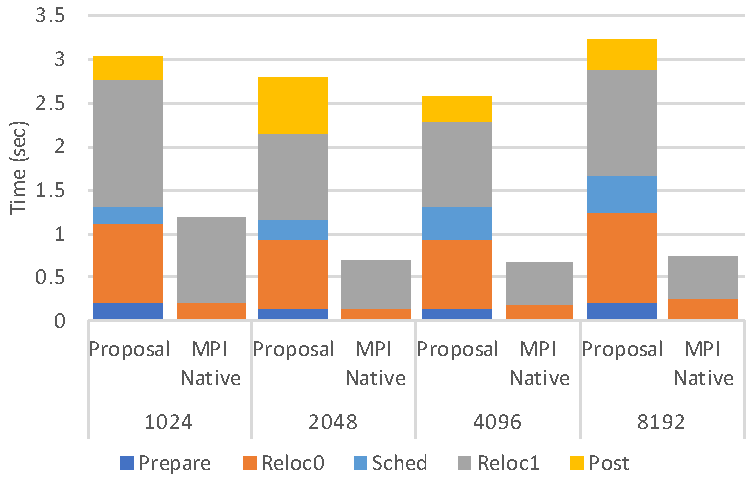
\includegraphics[width=0.7\textwidth]{eval_bqcd_ss.pdf}
  \caption{Comparison of overhead for data arrangement between our
    model and MPI Alltoall using BQCD: Strong Scalability}
  \label{takizawa_eval_bqcd_ss}
\end{figure}

\begin{figure}
  \centering
  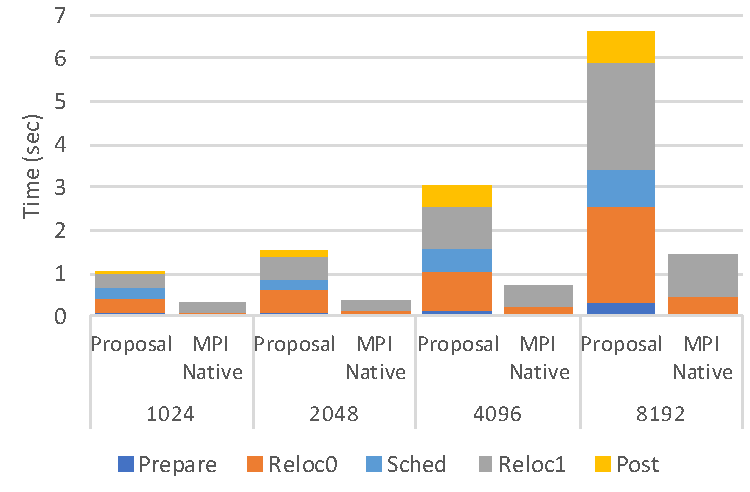
\includegraphics[width=0.7\textwidth]{eval_bqcd_ws.pdf}
  \caption{Comparison of overhead for data arrangement between our
    model and MPI Alltoall using BQCD: Weak Scalability}
  \label{takizawa_eval_bqcd_ws}
\end{figure}

\subsection{High Level Framework for High Performance AMR}
Adaptive Mesh Refinement methods reduce computational requirements of problems by increasing resolution for only areas of interest. However, in practice, efficient AMR implementations are difficult considering that the mesh hierarchy management must be optimized for the underlying hardware. Architecture complexity of GPUs can render efficient AMR to be particularity challenging in GPU-accelerated supercomputers. This work presents a compiler-based high-level framework that can automatically transform serial uniform mesh code annotated by the user into parallel adaptive mesh code optimized for GPU-accelerated supercomputers. Experimental results on three applications show that the speedups of code generated by our framework are comparable to hand-written AMR code, while achieving good and weak scaling up to 3,640 GPUs.
\subsubsection{Introduction}
In many scientific and engineering simulations, Partial Differential Equations (PDEs) are solved in a uniform mesh arrangement by using finite difference schemes, referred to as iterative stencils. Typically, the resolution of the mesh is uniformly set to the highest resolution to provide accurate solutions. For meshes that require only high resolution for some portions of the mesh, an alternative method, known as Adaptive Mesh Refinement (AMR), can be used instead of the uniform mesh. The AMR method solves the problem on a relatively coarse grid, and dynamically refines it in regions requiring higher resolution. However, AMR codes tend to be far more complicated than their uniform mesh counterparts due to the software infrastructure necessary to dynamically manage the hierarchical mesh framework. Despite this complexity, it is generally believed that future applications will increasingly rely on adaptive methods to study problems at unprecedented scale and resolution.
Implementing efficient adaptive meshes in GPU-accelerated systems is significantly hard in comparison to traditional CPU systems. More specifically, GPUs add complexity overhead for managing the mesh hierarchy and optimization of data movement. This is made evident by the relatively wide use of AMR in CPU in comparison to GPU-based systems. For example, a mature AMR framework supporting CPU, namely FLASH is reported to be in use by dozens of production applications~[1]. On the contrary, a few number of individual applications adapted AMR solvers for GPU, with varying levels of optimization and scaling. To summarize the problems with GPU-based AMR, only a few frameworks enable automated AMR transformations for GPU, and their programming models require the programmer to write his own versions of the target-optimized solvers. Moreover, there can be scalability limitations caused by the overhead of the CPU-GPU communication schemes in those frameworks~[2].
In this work, we present a high-level framework, called Daino~[3], which auto-generates efficient and scalable structured AMR solutions to scientific applications running on GPU-accelerated systems.
\subsubsection{Background}
Structured AMR methods use logically rectangular meshes in the implementation of the adaptive mesh. Structured AMR utilizes a hierarchy of levels of spatial, and often temporal, mesh spacing with each level being composed of a union of logically rectangular mesh regions. One way to represent the structured AMR, namely tree-based AMR, divides the discretized domain into fixed blocks. If any cell within a block requires refinement, the whole block is refined.
In the tree-based scheme, the mesh is organized into a hierarchy of refinement levels. The mesh is usually decomposed into relatively small fixed-sized octants of mesh cells. Each octant can be recursively refined into a set of octants of fine cells. The mesh configuration is managed using a tree-based data structure that maintains explicit child- parent relationships between coarse and fine octants. Size relations between neighboring octants are typically enforced in structured AMR, which means neighboring octants can have at most one level of refinement difference (referred to as 2:1 balance). An important feature of octrees is that the traversal of an octree across its leaves corresponds to a Morton z-shaped Space Filling Curve (SFC) in the geometric domain~[4]. Accordingly, sorting the blocks by their Morton ID and equally partitioning them leads to a uniform distribution of the blocks of a mesh among different Processing Elements (PEs), while benefiting from the locality provided by SFC affinity. Figure~\ref{fig:1} illustrates how the domain and tree are represented in AMR, and the use of SFC to divide the blocks among three PEs.
\begin{figure}[h]
\centering
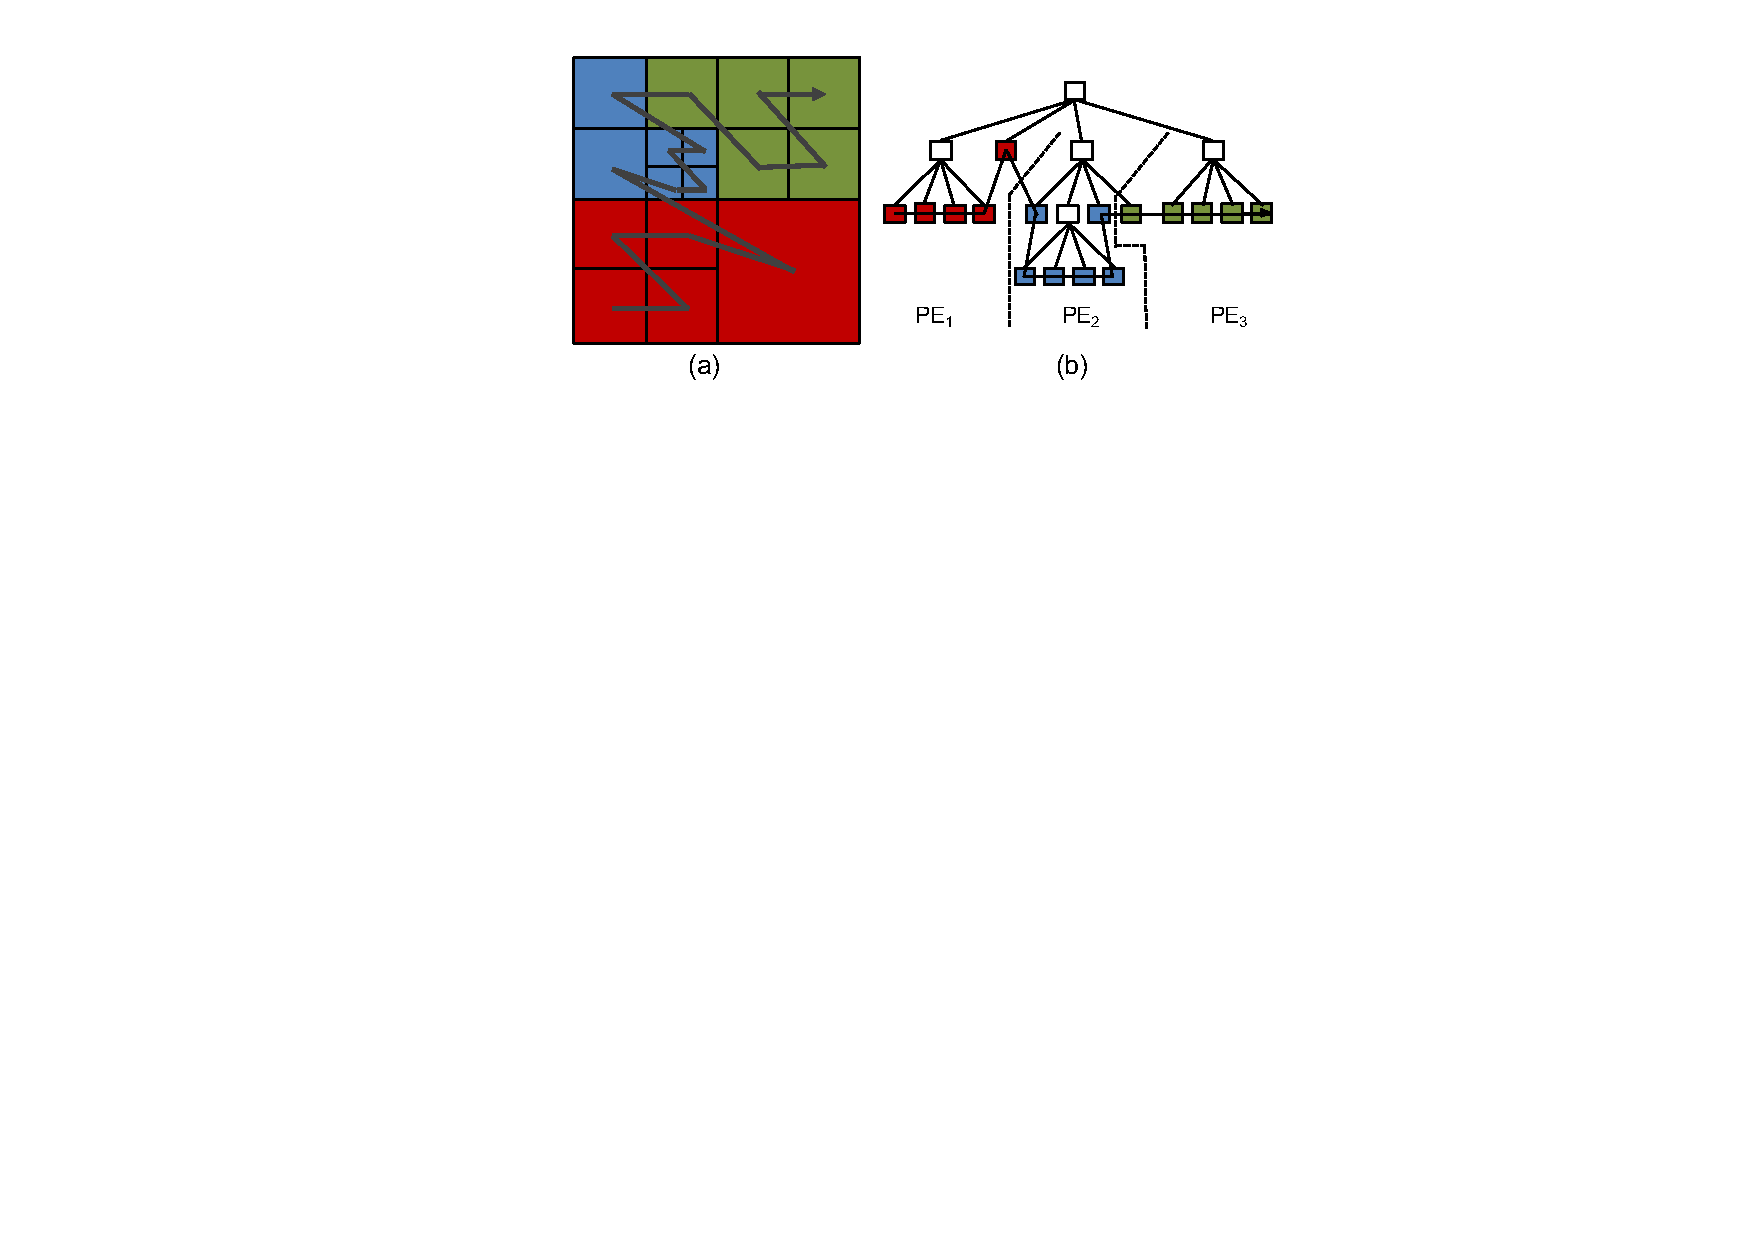
\includegraphics[width=0.8\textwidth]{figs/amr01.pdf}%1-expanded.pdf}%1.pdf}, 
\caption{Octree-based meshes. The blocks are equally partitioned into three PEs using a space filling curve. (a) Adaptive mesh (b) Tree representation (Note: 2D quadtree is used for illustration)}
\label{fig:1}
%%\vspace{-5pt}
\end{figure}
\subsubsection{High-level Framework for Efficient AMR}
We design a high-level programming framework that provides a highly productive programming environment for AMR. The framework is transparent and requires minimal involvement from the programmer, while generating efficient and scalable AMR code. The framework consists of a compiler and runtime components. A set of directives allows the programmer to identify stencils of a uniform mesh in an architecture- neutral way. The uniform mesh code is then translated to GPU-optimized parallel AMR code, which is then compiled to an executable. The runtime component encapsulates the AMR hierarchy and provides an interface for the mesh management operations.

\emph{Programming Model:} The framework provides directives to be used with standard C (details on directives in next section). The programmer is required to add the directives to a serial uniform mesh code in order to identify the operations and stencil data arrays that are the target for transformation. Note that the directives are not changing the uniform mesh implementation; the programmer can still use the uniform mesh implementation if the directives are ignored by compiler.

\emph{Optimizations:} When an AMR code generated by Daino is executed on a GPU-accelerated cluster, the stencil and mesh adaptation kernels run on the GPU, while managing the octree data structures and load balancing is done on the CPU side. Since we pursue efficiency and scalability, code on both the CPU and GPU should be optimized. The stencil operations in the blocks are themselves optimized for the GPU architecture~[5]. Other optimizations, such as data layout in memory and using user-managed cache memory, are applied on the GPU kernels responsible for adapting the mesh: error estimation, refinement (interpolation), and coarsening (extrapolation). Finally, the generated code includes optimizations to reduce the communication between nodes, i.e. boundary data exchange, and balancing the load, i.e. number of blocks per node.

\emph{Implementation:} Our framework consists of a compiler and runtime components. We generate executables optimized for GPU execution by leveraging the LLVM compiler infrastructure. The compiler builds on the LLVM compiler infrastructure~[6]. First, we use the front end to analyze and translate the stencil source code into GPU-optimized code in the form of LLVM Intermediate Representation (IR). Next, compiler passes are applied on the IR to add the AMR management code, which in turn make API calls to the runtime API and GPU-optimized code generated by the Nvidia backend code generator. Finally, LLVM IR is compiled and linked with the runtime libraries to generate and executable.
The runtime includes two libraries, the first library encapsulates the AMR hierarchy management software and the second is a communication library that wraps the MPI runtime library to simplify data movement operations for the AMR driver. The stages of compilation and layout of Diano are shown in Figure~\ref{fig:2}.
\begin{figure}[h]
\centering
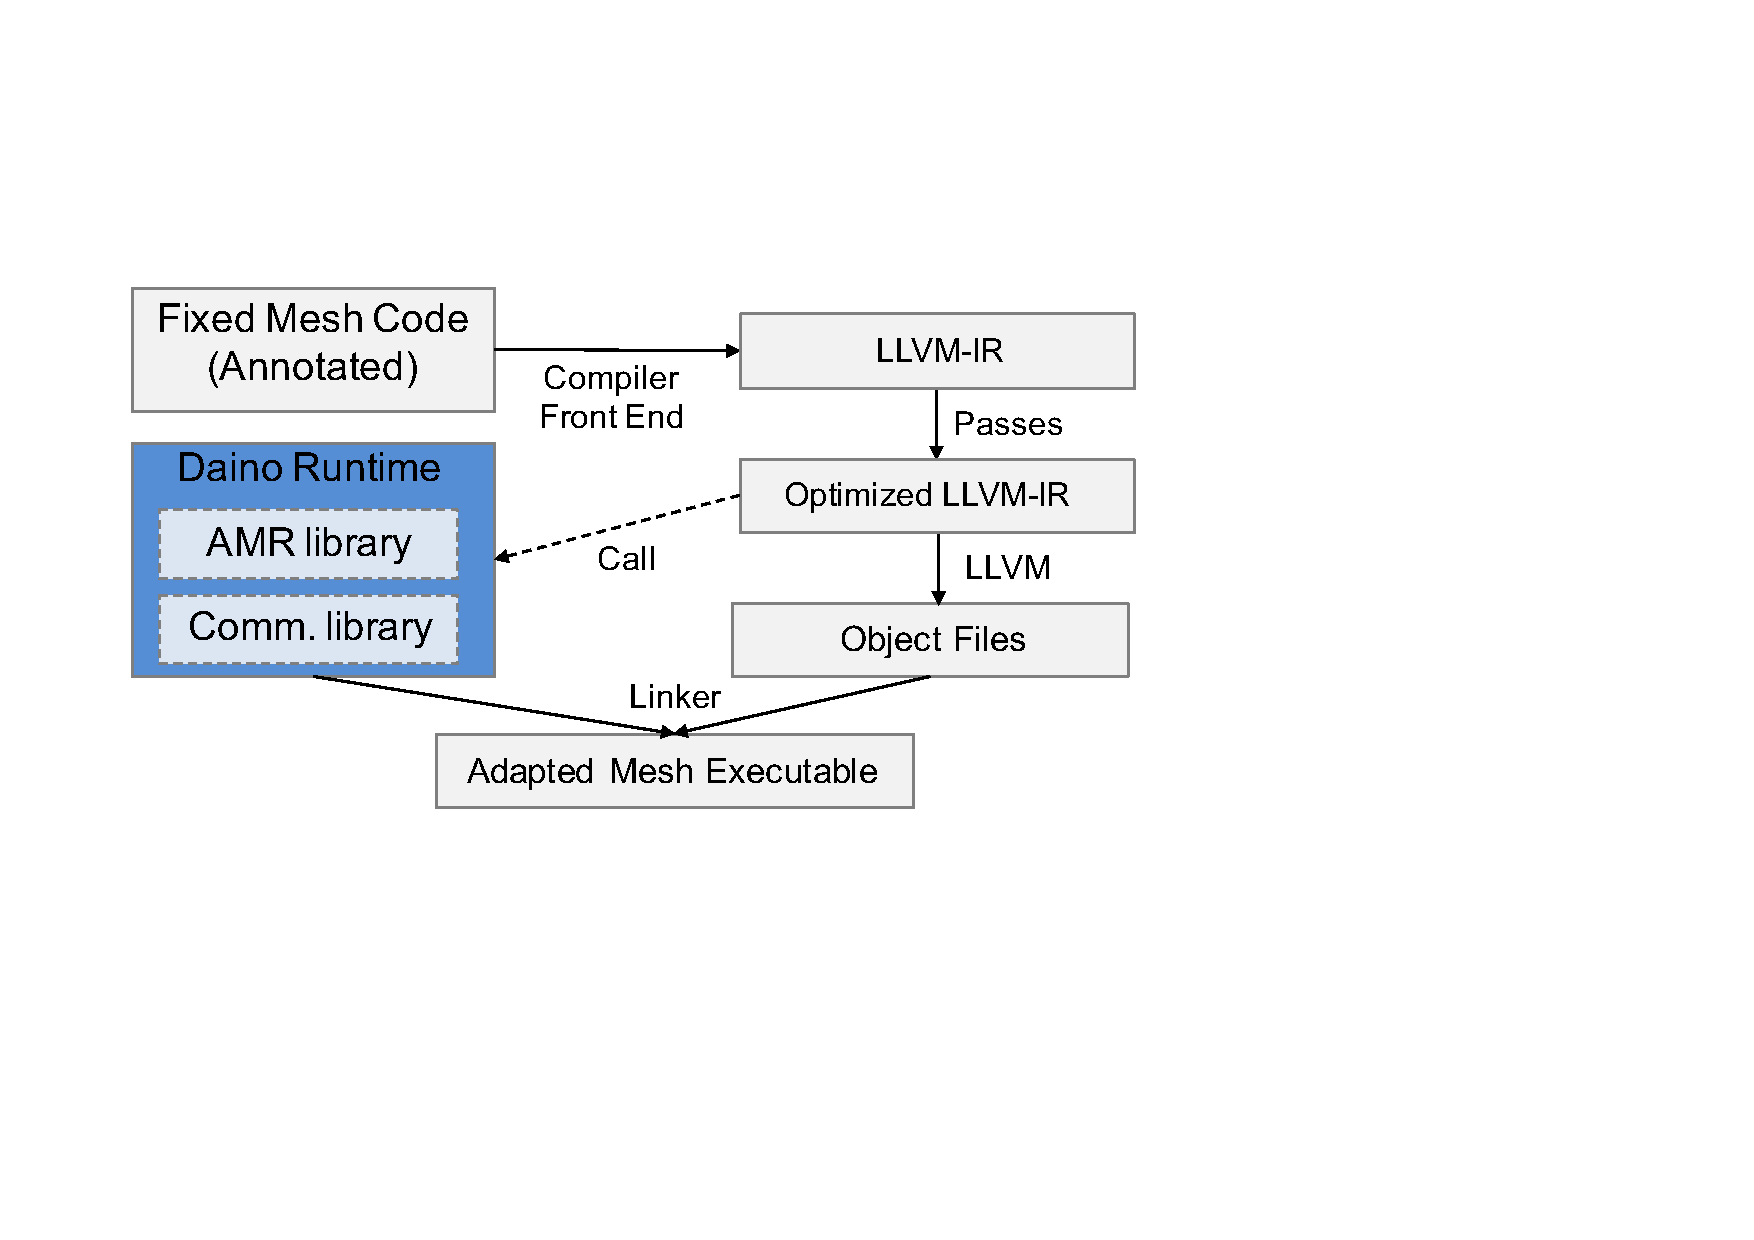
\includegraphics[width=0.8\textwidth]{figs/amr02.pdf}%1-expanded.pdf}%1.pdf}, 
\caption{The framework overview}
\label{fig:2}
%%\vspace{-5pt}
\end{figure}
\subsubsection{Evaluation}
We demonstrate the scalability of auto-generated AMR code using three production applications. We compare the speedup and scalability with hand-written AMR of all three applications. 

\emph{Applications:} a) Phase-field Simulation: This application simulates 3D dendritic growth during binary ally solidification~[7], b) Hydrodynamics Solver: This solver models a 2nd order directionally split hyperbolic schemes to solve Euler equations~[8], and c) Shallow-water: Modeling shallow water by depth-averaging Navier-Stokes equations~[9].

\emph{Results:} In a weak scaling experiment, shown in Figure~\ref{fig:3}, the run- time for uniform mesh, hand-written AMR, and auto-generated AMR are compared. The following points are important to note. First, more than 1.7x speedup is achieved using Daino suing the full TSUBAME machine, 3,640 GPUs, for the phase-field simulation. This is a considerable improvement considering that the uniform mesh implementation is a Gordon Bell prize winner for time-to- solution~[7]. Second, Daino achieves good scaling that comparable to the scalability of the hand-written AMR code.
\begin{figure}
\centering
\begin{subfigure}[t]{0.32\textwidth}
\centering
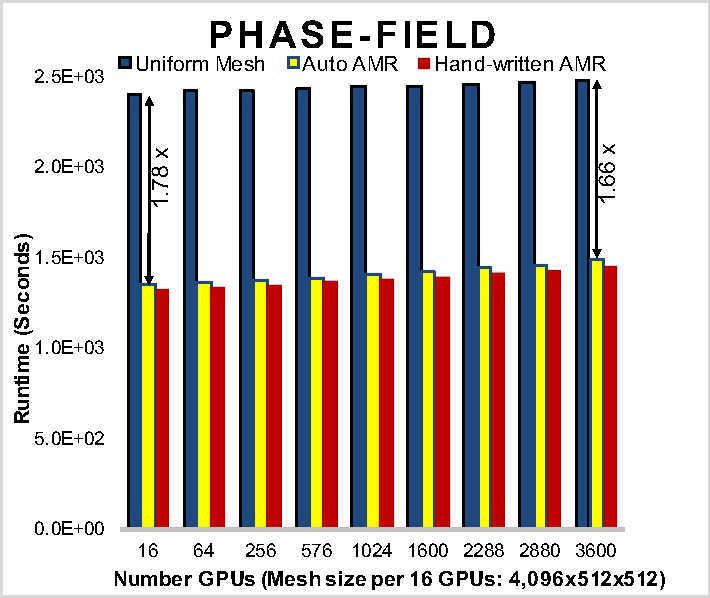
\includegraphics[width=\textwidth]{figs/amr03.pdf} 
\end{subfigure}
\begin{subfigure}[t]{0.32\textwidth}
\centering
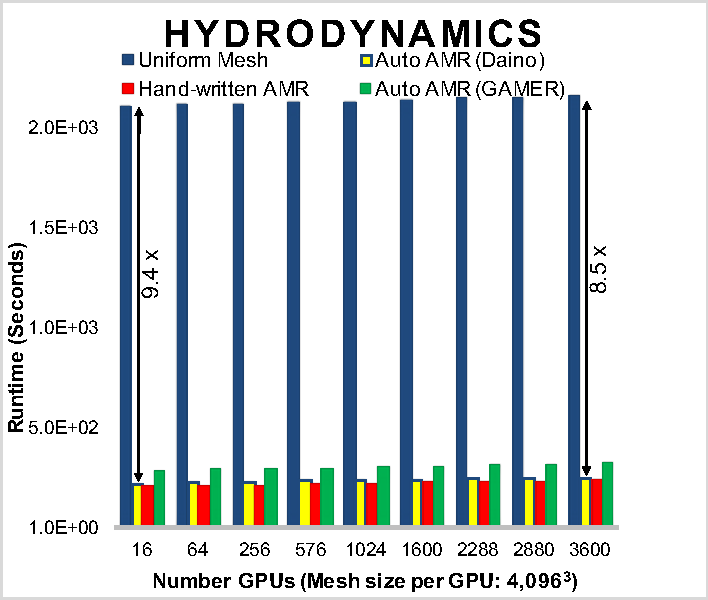
\includegraphics[width=\textwidth]{figs/amr04.pdf} 
\end{subfigure}
\begin{subfigure}[t]{0.32\textwidth}
\centering
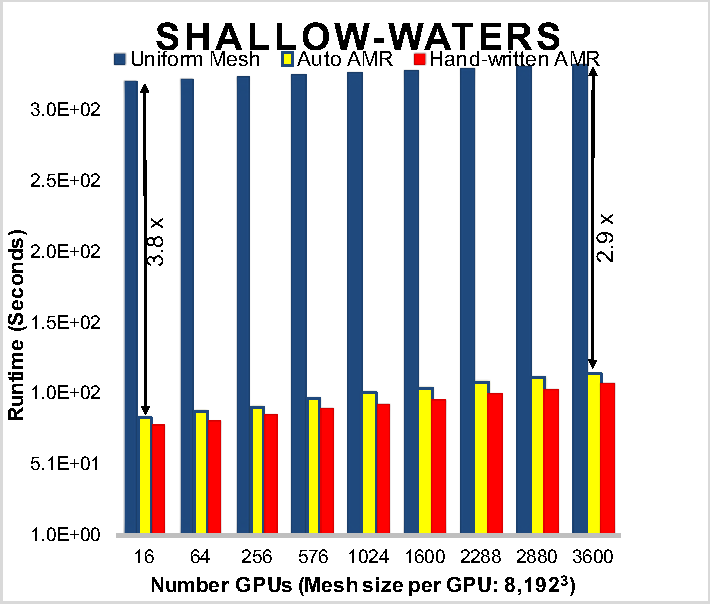
\includegraphics[width=\textwidth]{figs/amr05.pdf} 
 \end{subfigure}
\caption{Weak scaling of uniform mesh, hand-written and automated AMR}
\label{fig:3}
\end{figure}
Figure~\ref{fig:4} shows a strong scaling comparison for hand-written and auto-generated AMR against uniform mesh implementation. The code generated by Daino achieves speedups and scalability comparable to hand-written implementations. However, when using more GPUs, reduction in speedup starts to occur as the management of AMR starts to dominate the simulation runtime.
\begin{figure}
\centering
\begin{subfigure}[t]{0.32\textwidth}
\centering
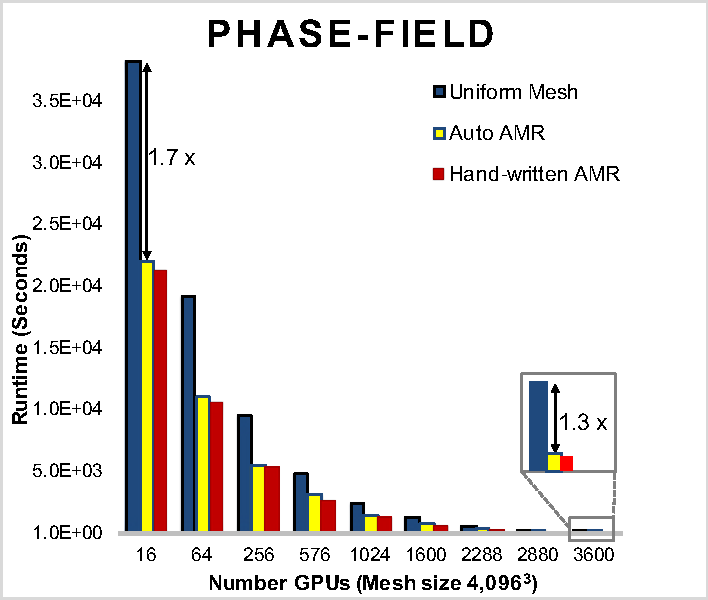
\includegraphics[width=\textwidth]{figs/amr06.pdf} 
\end{subfigure}
\begin{subfigure}[t]{0.32\textwidth}
\centering
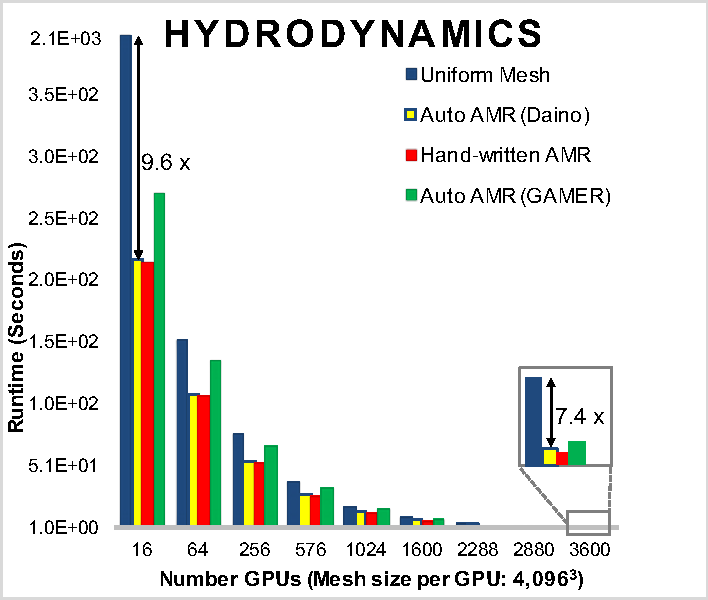
\includegraphics[width=\textwidth]{figs/amr07.pdf} 
\end{subfigure}
\begin{subfigure}[t]{0.32\textwidth}
\centering
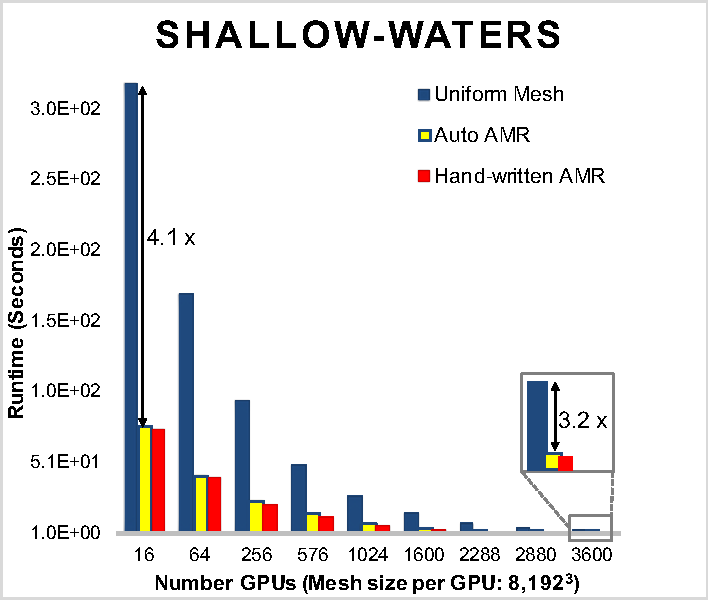
\includegraphics[width=\textwidth]{figs/amr08.pdf} 
 \end{subfigure}
\caption{Strong scaling of uniform mesh, hand-written and automated AMR}
\label{fig:4}
\end{figure}
\subsubsection{Summary}
Producing efficient AMR code is a challenge, especially for GPUs. We introduce a framework for producing efficient and distributed AMR code for GPU-accelerated systems. We demonstrated the efficacy and scalability of three applications using the full TSUBAME supercomputer. To the authors knowledge, this is the first study to scale auto-generated AMR code to O(1,000s) of GPUs. However, there are still problems to be solved, for example, handling of customized error functions and boundary conditions.
\subsubsection{References}
[1]~~A. Dubey, K. Antypas, M. K. Ganapathy, L. B. Reid, K. Riley, D. Sheeler, A. Siegel, and K. Weide, ‘’Extensible Component-based Architecture for FLASH, a Massively Parallel, Multiphysics Simulation Code,’’ Parallel Comp., vol. 35, no. 10-11, pp. 512–522, (2009) \newline
[2]~~M. Wahib, N. Maruyama, Data-centric GPU-based Adaptive Mesh Refinement, IA3 2015, Workshop on Irregular Applications: Architectures and Algorithms, co-located with SC’15, Austin, TX (2015) \newline
[3]~~M. Wahib, N. Maruyama, T. Aoki, Daino: A High-level Framework for Parallel and Efficient AMR on GPUs, SC'16, ACM/IEEE Proceedings of the International Conference for High Performance Computing, Networking, Storage and Analysis (2016) \newline
[4]~~H. Tropf and H. Herzog, ‘’Multidimensional Range Search in Dynamically Balanced Trees,’’ Angewandte Informatik, 1981 (1981) \newline
[5]~~N. Maruyama and T. Aoki, Optimizing Stencil Computations for NVIDIA Kepler GPUs, 1st International Workshop on High-Performance Stencil Computations HiStencils'14 (2014) \newline
[6]~~http://www.llvm.org \newline
[7]~~T. Shimokawabe, T. Aoki, T. Takaki, T. Endo, A. Yamanaka, N. Maruyama, A. Nukada, and S. Matsuoka, ‘’Peta-scale Phase-field Simulation for Dendritic Solidification on the TSUBAME 2.0 Supercomputer,’’ ser. SC ’11 (2011)  \newline
[8]~~H.-Y. Schive, U.-H. Zhang, and T. Chiueh, ‘’Directionally Unsplit Hydrodynamic Schemes with Hybrid MPI/OpenMP/GPU Parallelization in AMR,’’ Int. J. High Perform. Comput. Appl., vol. 26, no. 4, pp. 367–377 (2012)  \newline
[9]~~M. Sætra, A. Brodtkorb, K. Lie, ‘’Efficient GPU-implementation of Adaptive Mesh Refinement for the Shallow-Water Equations,’’ J. Sci. Comput., vol. 63, no. 1, pp. 23–48 (2015)


\subsection{Extending a Global Climate Model with a High Level Framework}
Mature climate models are complex codebases comprised of different components each with its own requirements and specifics. As we transition into the complex, and diverse, architectures of next-generation supercomputers, optimizing and adapting each of those components becomes more challenging. An additional challenge is to assure that those optimized components will seamlessly work together, in a performance portable fashion. In this work, we investigate a path for transitioning climate models to next-generation supercomputer, which an emphasize on performance profitability and end-user productivity. More specifically, We aim to demonstrate how to approach and integrate each of the components of an atmospheric model, NICAM. For porting the entire dynamical core, we use a C++ framework developed by the Swiss National Supercomputing Center, named GridTools, that could produce highly performing code for different target architectures. For the physical parameterization component, we propose a user-friendly Python-based approach to assure high productivity and practicality; physical parameterization code is typical continuously changed, unlike the dynamical core. It is important to note is that performance portability is a main concern we try to address in this work; next-generation supercomputers have high diversity in architectures. 

\subsubsection{Porting NICAM-DC 2016 Benchmark}
To evaluate the productivity and performance of GridTools, we extracted seven kernels from the dynamical core of NICAM (publicly available at: \url{https://github.com/hisashiyashiro/nicam_dckernel_2016}). We found that the performance for three benchmarks is comparable to hand-written CUDA code. Performance in comparison to hand-written OpenMP code for CPU is also found to be satisfactory. Based on the promising results, we continue to port the dynamical core of NICAM to GridTools.


\section{Schedule and Future Plan}


For the scalable multi-granular data model, we plan to improve the implementation to further reduce overhead and apply it to other applications, such as weather prediction. For the global climate model study, we plan to continue the study of the effectiveness of high level frameworks such as GridTools.


\section{Publications}

\subsection{Journal Articles}

\subsection{Conference Papers}

[1] Shinichiro Takizawa, Motohiko Matsuda, Naoya Maruyama, Yoshifumi Nakamura. A Scalable Multi-Granular Data Model for Data Parallel Workflows. HPC Asia 2018. 2018 (submitted). \newline
[2] M. Wahib, N. Maruyama, T. Aoki, Daino: A High-level Framework for Parallel and Efficient AMR on GPUs, SC'16, ACM/IEEE Proceedings of the International Conference for High Performance Computing, Networking, Storage and Analysis (2016) \newline

\subsection{Posters and Presentations}
[3] M. Wahib, Invited Talk: “Daino: A High-level Framework for Parallel and Efficient AMR on GPUs”, Argonne National Laboratory, December 2016
RIKEN AICS (PADAL Workshop) \newline
[4] Shinichiro Takizawa, Motohiko Matsuda, Naoya Maruyama. A Locality-aware Task Scheduling of Message Passing and MapReduce Hybrid Models. HPDC 2016 Poster. 2016. \newline
[5] M. Wahib, Invited Talk: "Automatically Fusing Hundreds of Stencil Kernels for Better Performance and Productivity”, GTC 2016 (Nvidia GPU Technology Conference) \newline

\subsection{Patents and Deliverables}

\part{Operations and Computer Technologies Division}

\chapter{... Team}

\section{Members}

\section{Research Activities}

\section{Research Results and Achievements}

\subsection{Subject A...}

\subsection{Subject B...}

\section{Schedule and Future Plan}

\section{Publications}

\subsection{Journal Articles}

\subsection{Conference Papers}


\subsection{Posters and Presentations}


\subsection{Patents and Deliverables}



\part{Flagship 2020 Project}


\chapter{Flagship 2020 Project}

\end{document}




